%!TEX root = draft.tex

\section{Attributed Random Walk Model}
\label{sec:Proposed Model}
The Attributed Random Walk (\texttt{ARW}) model explains the emergence
of key structural properties of real networks through local edge formation mechanisms.
First, we describe the edge formation mechanisms underlying \texttt{ARW}. Then,
we briefly discuss the methods required to fit the model to data.


\subsection{Model Description}
\label{sub:Model Description}

\texttt{ARW} grows a directed network over time as new nodes join the network.
The mechanism that nodes use to form edges intuitively corresponds to how we
expect researchers to conduct a literature survey and cite relevant work.
First, the researcher broadly identifies \textit{relevant} papers,
possibly with the help of external information sources.
Then, under time and information constraints, the individual navigates a chain
of references to identify \textit{similar} papers that either support or
address the problem in hand.  Next, through careful analysis, he or she
decides to cite a subset of these papers; Heuristics such as number of
citations maybe used in the decision making process.
Incoming nodes in \texttt{ARW} use a similar mechanism to form edges.
New nodes select a seed node and initiate a random walk to (a) explore the network
by navigating through neighborhoods of existing nodes and (b) probabilistically
link to visited nodes based on attribute similarity, as shown in \Cref{fig:randomwalk}.

The Attributed Random Walk (\texttt{ARW}) model grows a directed network $\{G_t\}^T_{t=1}$.
More formally, at every discrete time step $t$, a
new node $u$, with attribute value $A(u)$, joins the network $G_t=(V_t, E_t,
A_t)$, where $V_t, E_t$ and $A_t$ are sets of nodes, edges and unique attribute
values at time $t$. After joining the network, node $u$ forms $m(t)$ edges to
existing nodes. At time $t$, $G_t$ consists of ${|V_t|=|V_0|+t}$ nodes,
${|E_t|=|E_{t-1}|+m(t)}$ edges and the set of attribute values ${A_t = A_{t-1}
\cup \{A(u)\}}$.
% Outdegree $m(t)$ of incoming nodes increases over time to
% reflect the nonlinear growth and densification of real networks.
We discuss the
issue of initializing $G_0$, sampling attribute value $A(u)$ and modeling
densification using $m(t)$ in \Cref{sub:Model Fitting}.

The edge formation mechanism consists of two components: \textsc{Select-Seed} and
\textsc{Random-Walk}. A new node $u$ with attribute value $A(u)$ that joins the
network at time $t$ first selects a seed node $s_u$ using \textsc{Select-Seed}:
\\\\
\tikzstyle{background rectangle}=[thin,draw=black]
\begin{tikzpicture}[show background rectangle]
\node[align=left, text width=.93\linewidth, inner sep=.5em]{
(1) With probability $p_a$, randomly select $s_u$ from the set of existing nodes that have attribute
value $A(u)$.

\vspace{1mm}
(2) Otherwise, with probability $1-p_a$, randomly select $s_u$ from the set of existing nodes that
do \textit{not} have attribute value $A(u)$.
};
\node[xshift=3ex, yshift=-.7ex, overlay, fill=white, draw=white, above
right] at (current bounding box.north west) {
\textsc{Select-Seed}
};
\end{tikzpicture}

% The attribute parameter $p_a$ incorporates the attribute preferences of incoming nodes
% into the model.
In \textsc{Seed-Select}, attribute parameter $p_a$ is the probability with which
an incoming node and its seed node have the same attribute value.
% As shown in \Cref{fig:randomwalk}, node $u$ has homophilic preferences if $p_a$ is greater than the fraction of existing nodes with attribute value $A(u)$.
After selecting the seed $s_u$, node $u$ initiates a random walk using
\textsc{Random-Walk} to form $m(t)$ links:
\\\\
\tikzstyle{background rectangle}=[thin,draw=black]
\begin{tikzpicture}[show background rectangle]
\node[align=left, text width=.93\linewidth, inner sep=.5em]{
(1) At each step of the walk, new node $u$ visits node $v_i$.
    \begin{itemize}
        \item If $A(u)=A(v_i)$, $u$ links to $v_i$ with probability $\alpha \cdot p_a$
        \item Otherwise, $u$ links to $v_i$ with probability $\alpha \cdot (1-p_a)$
    \end{itemize}

\vspace{1mm}
(2) Then, with probability $p_j$, $u$ jumps back to seed $s_u$.

\vspace{1mm}
(3) Otherwise, with probability ${1-p_j}$, $u$ continues to walk. It picks an outgoing edge with probability $p_o$ \textit{or}
an incoming edge with probability $1-p_o$ to visit a neighbor of $v_i$.

\vspace{1mm}
(4) Steps 1-3 are repeated until $u$ links to $m(t)$ nodes.
};
\node[xshift=3ex, yshift=-.7ex, overlay, fill=white, draw=white, above
right] at (current bounding box.north west) {
\textsc{Random-Walk}
};
\end{tikzpicture}

Random walks inherently account for limited information and partial network access as
they only require information about the neighborhood of visited nodes.
\begin{figure}[h]
    \centering
    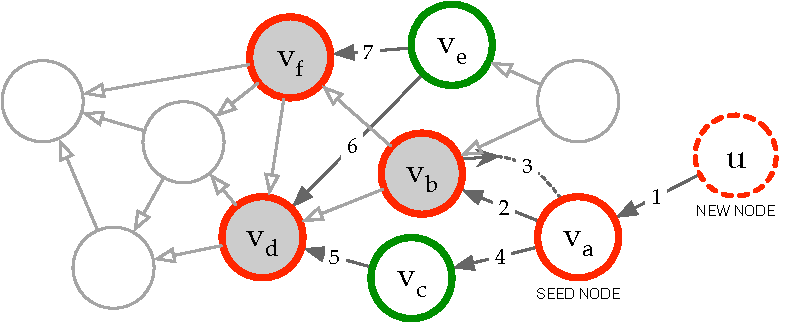
\includegraphics[width=.9\linewidth]{random_walk}
    \vspace{3mm}
    \caption{Edge formation in \texttt{ARW}.
    A new node $u$ joins the attributed network with outdegree ${m=3}$ and attribute value
    {$A(u)=\textsc{red} \in \{\textsc{red},\textsc{blue}\}$}.
    It uses \textsc{Select-Seed} to select seed node $v_a$ and initiates a \textsc{Random-Walk}.
    As denoted by the labeled edges, node $u$ starts from $v_a$, moves to $v_b$, jumps back to seed $v_a$ and
    visits $v_c, v_d, v_e$ and $v_f$. It links to three nodes ---  $v_b$, $v_d$ \& $v_f$ ---
    that have the same attribute value.}
    \label{fig:randomwalk}
    \vspace{-2mm}
\end{figure}

The \textsc{Random-Walk}
mechanism consists of four parameters - $\alpha$ \& $p_a$
parameterize edge formation decisions and $p_j$ \& $p_o$ characterize random walk
traversals:
\begin{itemize}
    \item The rate parameter $\alpha$ controls the rate at which $u$ links to
    visited nodes; It implicitly incorporates triadic closure because the
    probability that node $u$ ``closes'' a triad by linking to an existing node
    $v_i$ and its neighbors is proportional to $\alpha^2$.

    \item The attribute parameter $p_a$ accounts
    for homophily/heterophily by incorporating attribute preferences of incoming nodes
    into the model.

    \item The jump parameter $p_j$ is the probability with which $u$ restarts the
    random walk from seed $s_u$; It controls the extent to which structural constraints restrict $u$ to link to nodes that are
    structurally proximate and in the same locality.

    \item The out parameter $p_o$ is the probability with which a node chooses an
    outgoing edge in its random walk traversal. Incoming nodes can visit old nodes
    by randomly traversing the network using \textit{outgoing} edges because an
    edge from $u$ to $v$ exists iff $u$ joins the network after $v$. Moreover,
    random walk models \cite{vazquez2000knowing} exhibit positive correlation between node
    indegree and node age observed in real networks.
    As a result, $p_o$ incorporates bias towards high
    degree nodes by controlling the rate at which incoming nodes approach old nodes.
\end{itemize}

In the absence of attribute data, the edge formation mechanisms are further simplified
because the attribute parameter $p_a$ is not required. \textsc{Seed-Select} simplifies
to selecting an existing node uniformly at random and edge formation in \textsc{Random-Walk}
depends on the rate parameter $\alpha$ only.

To summarize, the Attributed Random Walk (\texttt{ARW}) model
intuitively describes how individuals form edges under resource constraints.
\texttt{ARW} uses four parameters --- $\alpha$, $p_a$, $p_j$, $p_o$ --- to incorporate
individuals' biases towards similar, proximate and high degree nodes.

\subsection{Model Fitting}
\label{sub:Model Fitting}
We now briefly describe methods to estimate \texttt{ARW} parameters,
initialize $\hat{G}$ at time ${t=0}$, densify $\hat{G}$
over time and sample incoming nodes' attribute values.

\textit{Parameter Estimation}.
The rate parameter $\alpha$, attribute parameter $p_a$, jump parameter $p_j$ and
out parameter $p_o$ jointly control the edge formation mechanism in \texttt{ARW}.
These parameters subsequently determine the structural properties of the network $\hat{G}$
generated by \texttt{ARW}. The parameter estimation task consists of finding the set of
parameters values for $(\alpha, p_a, p_j, p_o)$ that best explain the structural properties
of an observed network $G=(V,E,A)$. We use a straightforward grid search method to estimate
the four parameters. We describe the evaluation metrics and selection criteria in \Cref{sub:Experimental Setup}.
Other derivative-free optimization methods such as the Nelder-Mead method can be used to quicken parameter estimation.

\textit{Initialization}. The edge formation mechanism in \texttt{ARW} is
sensitive to a large number of weakly connected components \texttt{WCC}s in the
initial network $\hat{G}_0$ because incoming nodes can only form edges to nodes
in the same \texttt{WCC}. To ensure that $\hat{G}_0$ is weakly
connected, we perform an undirected breadth-first search on the observed,
to-be-fitted network $G$ that starts from the oldest node and terminates after
visiting $0.1$-$1\%$ of the nodes. The initial network $\hat{G}_0$ is the small
subgraph induced from the set of visited nodes.
% Simpler initialization methods
% such as sampling $\hat{G}_0$ from the Erdos-Renyi model or Watts-Strogatz model
% yield similar results.

\textit{Densification}. In \cref{sec:Analysis}, we observed that real
networks densify over time, with the number of edges growing superlinearly in
the number of nodes. We incorporate densification into \texttt{ARW} by
increasing the outdegree of new nodes that \textit{sequentially} join the
network $\hat{G}$.
Each incoming node $u$ that joins $\hat{G}$ at time $t$ corresponds to some
 node that joins the observed network $G$ in
year $y(t)$; The number of edges $m(t)$ that $u$ forms is equal to the average
outdegree of nodes that join $G$ in year $y(t)$. Therefore, the rate of growth
in $\hat{G}$ coarsely reflects the rate of growth in $G$.

\textit{Sampling Attribute Values}. In real networks $G=(V,E,A)$,
the distribution over the set of attribute values $P_{\textsc{g}}(A)$ changes over time.
For instance, the attribute distribution over journals in the \texttt{APS} citation
network changes over time as old journals decay in popularity and new journals gain traction.
To incorporate this phenomenon into \texttt{ARW}, we sample the attribute value $A(u)$ of node $u$, that
joins $\hat{G}$ at time $t$, from $P_{\textsc{g}}(A{\mbox{ | year}=y(t)})$, the observed attribute distribution
conditioned on the corresponding year of node $u$.


In this section, we described the Attributed Random Walk
model and discussed methods related to model fitting. Next, our experiments in
\cref{sec:Experiments} show that $\texttt{ARW}$ accurately preserves
\textit{multiple} structural properties of real networks
% \Cref{sec:Experiments}, we show that the cumulative effect of the edge
% formation processes in \texttt{ARW} --- triadic closure, strong homophily,
% structural constraints and preferential attachment --- explains the emergence
% of high clustering, assortative mixing and heavy tailed degree distributions in
% real networks.

% The goal of our resource-constrained
% model is to generate networks that follow structural properties of real networks
% discussed in~\Cref{sec:Empirical Analysis}.
% Third, we show that
% \texttt{ARW} intrinsically incorporates local processes --- preferential
% attachment, triadic closure and homophily --- that effect edge formation in real
% networks.

% \subsection{Empirical Observations}
% \label{sub:Empirical Observations}
%
% \texttt{ARW} grows a directed network over time as new nodes join the network.
% The mechanism that nodes use to form edges intuitively corresponds to how we
% expect researchers to conduct a literature survey and cite relevant work.
% First, the researcher broadly identifies \textit{relevant} papers.
% possibly with the help of external information sources.
% Then, under time and information constraints, the individual navigates a chain
% of references to identify \textit{similar} papers that either support or
% address the problem in hand.  Next, through careful analysis, he or she
% decides to cite a subset of these papers; Heuristics such as number of
% citations maybe used in the decision making process.
%
% Incoming nodes in \texttt{ARW} use a similar mechanism to form edges.
% New nodes select a seed node and initiate a random walk to (a) explore the network
% by navigating through neighborhoods of existing nodes and (b) probabilistically
% link to visited nodes based on attribute similarity, as shown in \Cref{fig:randomwalk}.
% The following observations guide the development of the Attributed Random Walk model.
% \vspace{-2mm}
% \begin{enumerate}
%     \item \textbf{Proximity \& homophily}: Sociological studies \cite{35626,block2014multidimensional,mcpherson2001birds} on
%     evolving social networks indicate that both, structural proximity and
%     homophily, are important factors that influence edge formation. Homophilic
%     preferences cause similarity-induced edge formation whereas structural
%     factors act as constraints that restrict opportunities to structurally proximate
%     nodes (e.g. friend of a friend).
%
%     \item \textbf{Biased human navigation}: Analysis \cite{west2012human} of Wikispeedia \cite{west2009wikispeedia},
%      a game in which players must navigate from page \texttt{X} to page
%     \texttt{Y} using as few hyperlinks as possible, sheds light on how individuals
%     navigate networks with limited, \textit{local} information. Their
%     findings indicate that individuals (a) move to well-connected, high-degree pages
%     that maximize information and (b) rely on pages' content attributes to reach \texttt{Y}.
%
%     \item \textbf{Decision making under constraints}: Individuals make edge
%     formation decisions based on limited information and
%     partial network access.
%     For example, a researcher cites references without
%     knowing or having access to all papers in her field.
% \end{enumerate}
%
%
% Based on these observations, an edge formation mechanism should account for bias
% towards nodes that are similar, proximate or well-connected. It should also
% incorporate resource constraints to model how individuals form
% edges in real networks.
% % Nodes in \texttt{ARW} use random walks to
% % explore the network and link to existing nodes concurrently.
% % Random walk traversals only require information about the neighborhood of a small subset of visited nodes.
% Next, we describe the edge formation mechanism in \texttt{ARW}.


% \subsection{Parameter Space}
% \label{sub:Parameter Space}
%
% In this subsection, we study the variability in the structural properties of
% networks generated by our model. We also show that each model parameter
% is necessary because it influences different aspects of global network
% structure.

